\documentclass[a4paper,12pt]{scrartcl}

\usepackage{graphicx}


\usepackage[ngerman] {babel}
\usepackage[T1]{fontenc}
\usepackage{float}
\usepackage[utf8]{inputenc}
\usepackage{fancyhdr}
\pagestyle{fancy}

\lhead{1}
\chead{2}
\rhead{3}

\lfoot{4}
\cfoot{5}
\rfoot{6}


\setlength{\parindent}{0em} 

\title{Diplomarbeit}
\author{Dominik Pichler}
\date{21. Jänner 2018}

\begin{document}

\maketitle
\tableofcontents
\setcounter{tocdepth}{3}

\section{Teil 1 Mechanik}
\subsection{Einleitung}
\subsection{Aufgabenstellung}
\subsubsection{Zielsetzung}
\subsubsection{Problematik}
\subsection{Konzepte} \newpage



\subsubsection{Variante 1} 
\textbf{Übersicht der Prozessschritte:}
\begin{itemize}
\item[1] Füllen des Futtermagazins
\item[2] Führen zur Schneidplatte
\item[3] Schnitt
\item[4] Pressen
\item[5] Entsorgen
\item[6] Füttern
\end{itemize}

\textbf{1.Füllen des Futtermagazins:} \\

Im folgenden Bild wird mithilfe einer Lego-Darstellung gezeigt, wie das Magazin aus verschiedenen Blickwinkeln befüllt aussieht. Hier muss man beachten das die vom Hersteller zu öffneten Seite in Richtung des Schneidewerks zeigt (die schmale Seite mit der Einkerbung).

\begin{figure}[H]
\begin{center}
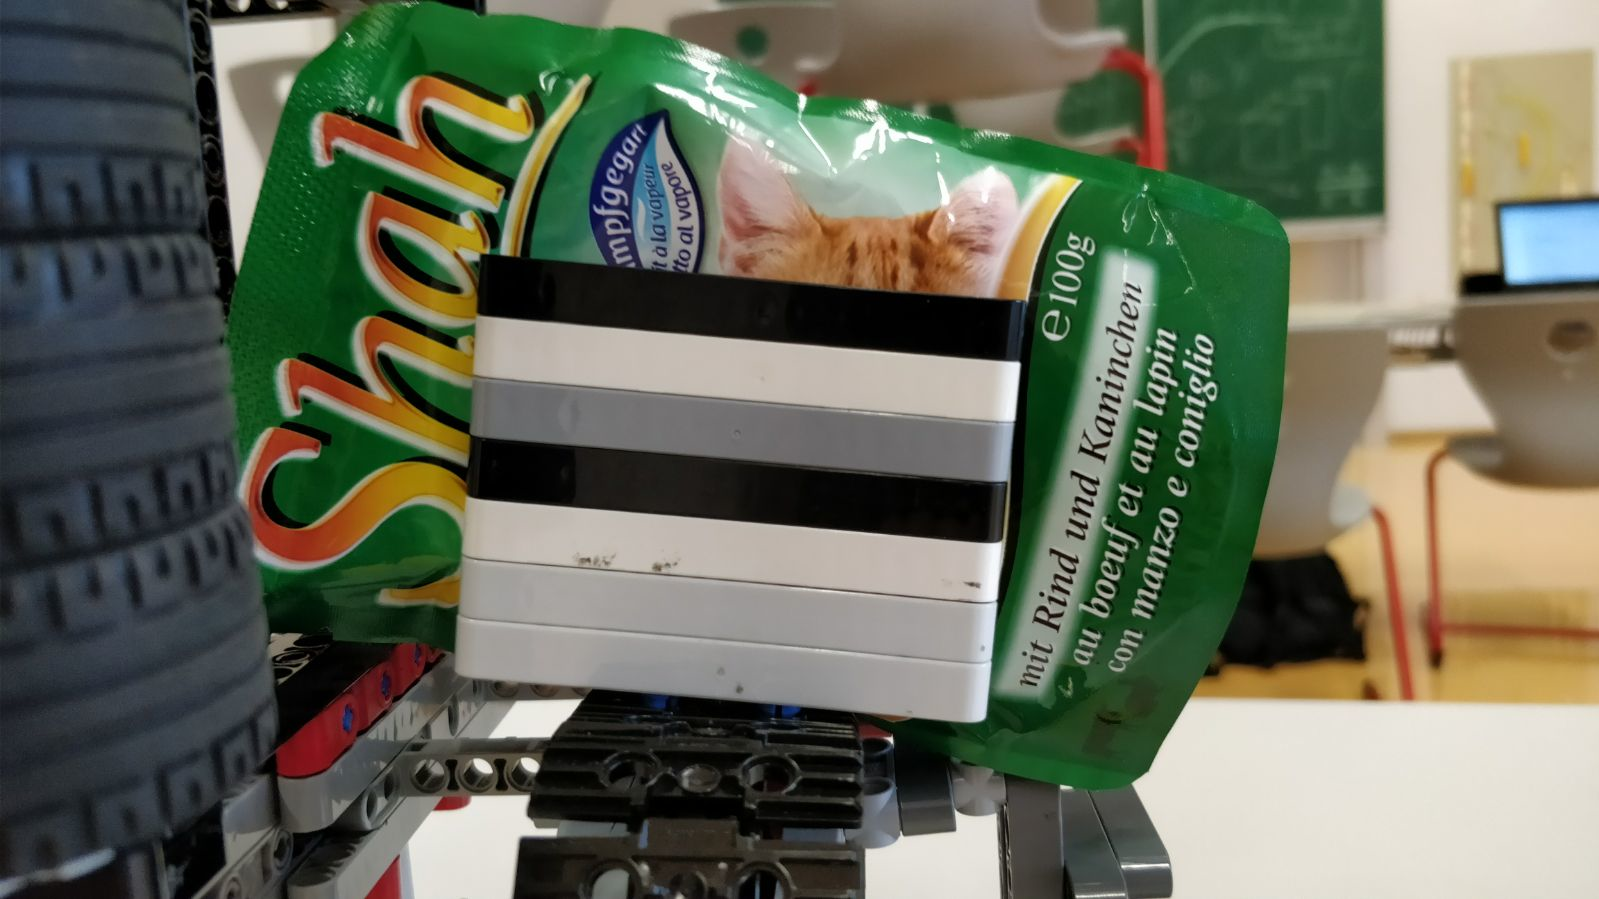
\includegraphics[width=13cm]{Bilder/Ablauf_1_png/Magazin_Vorne.png}
\caption{Magazin Vorne}
\end{center}
\end{figure}

\begin{figure}[H]
\begin{center}
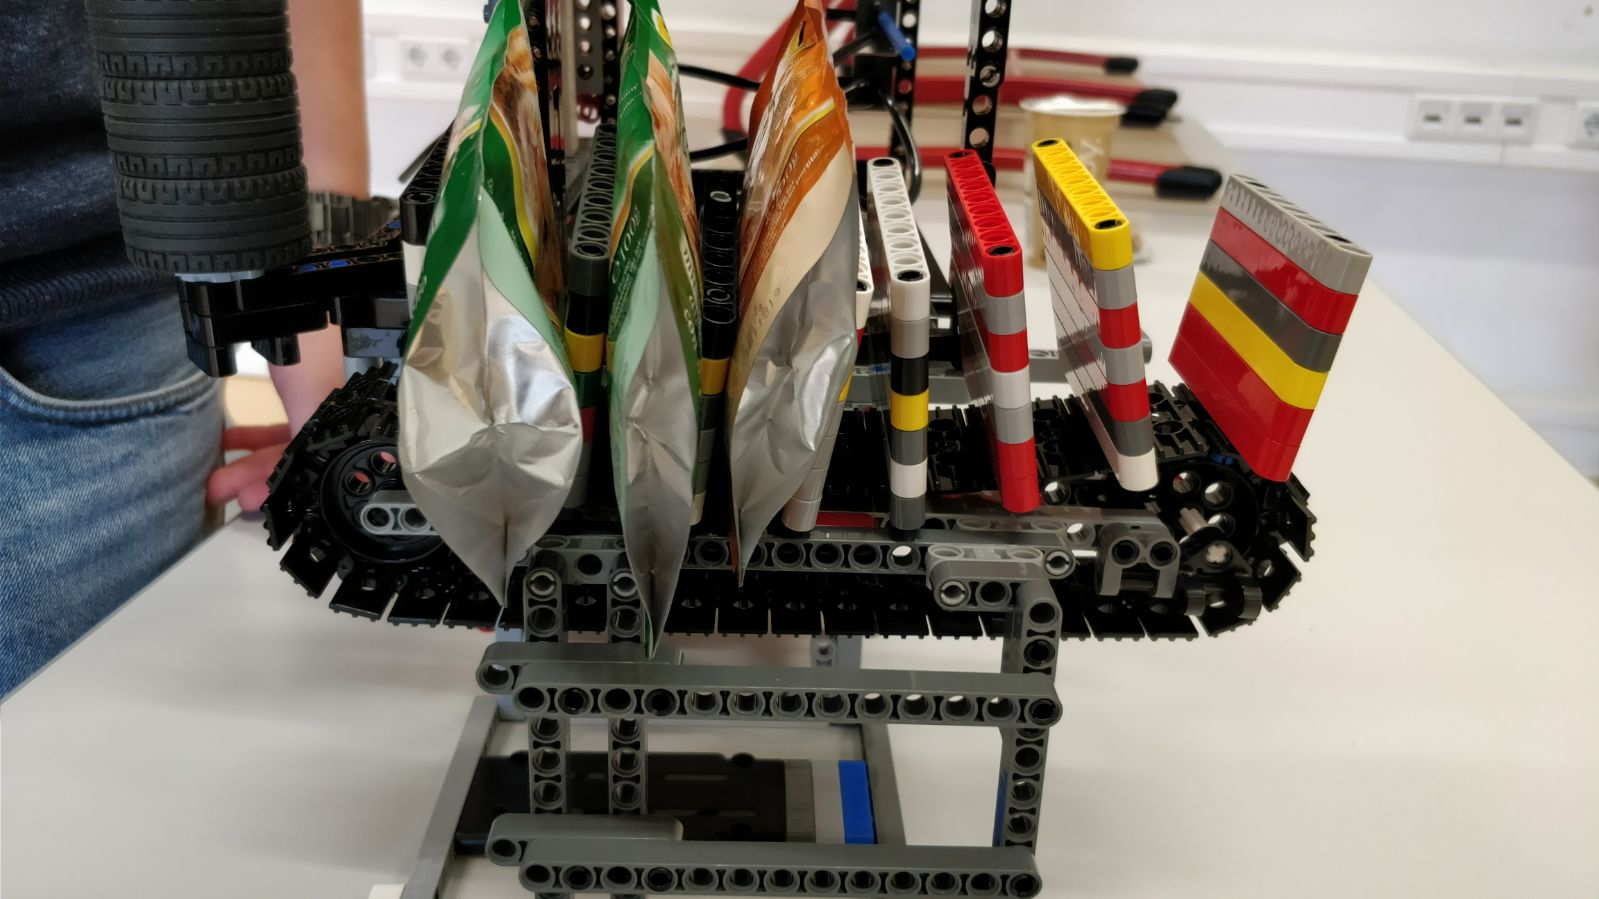
\includegraphics[width=13cm]{Bilder/Ablauf_1_png/Magazin_Seitlich.png}
\caption{Magazin Seitlich}
\end{center}
\end{figure}

\begin{figure}[H]
\begin{center}
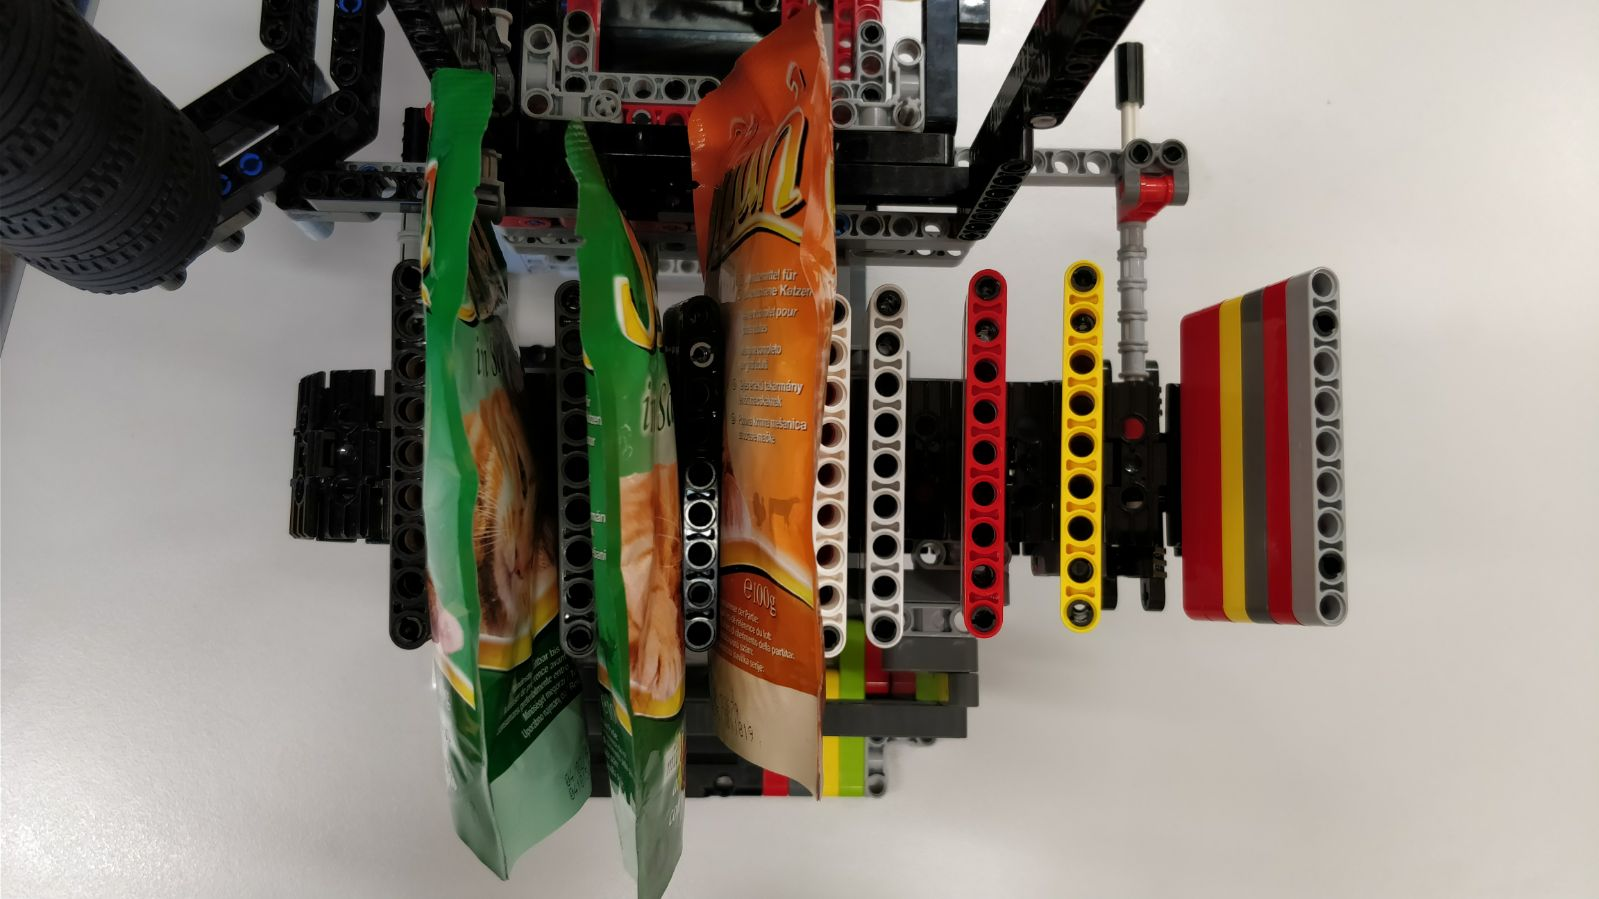
\includegraphics[width=13cm]{Bilder/Ablauf_1_png/Magazin_Oben.jpeg}
\caption{Magazin Oben}
\end{center}
\end{figure}

\newpage 

\textbf{2.Führen zur Schneidplatte:} \\ 

In diesem Schritt wird mithilfe eines Greifers (dargestellt durch eine Hand) die Packung in richtiger Position gebracht.

\begin{figure}[H]
\begin{center}
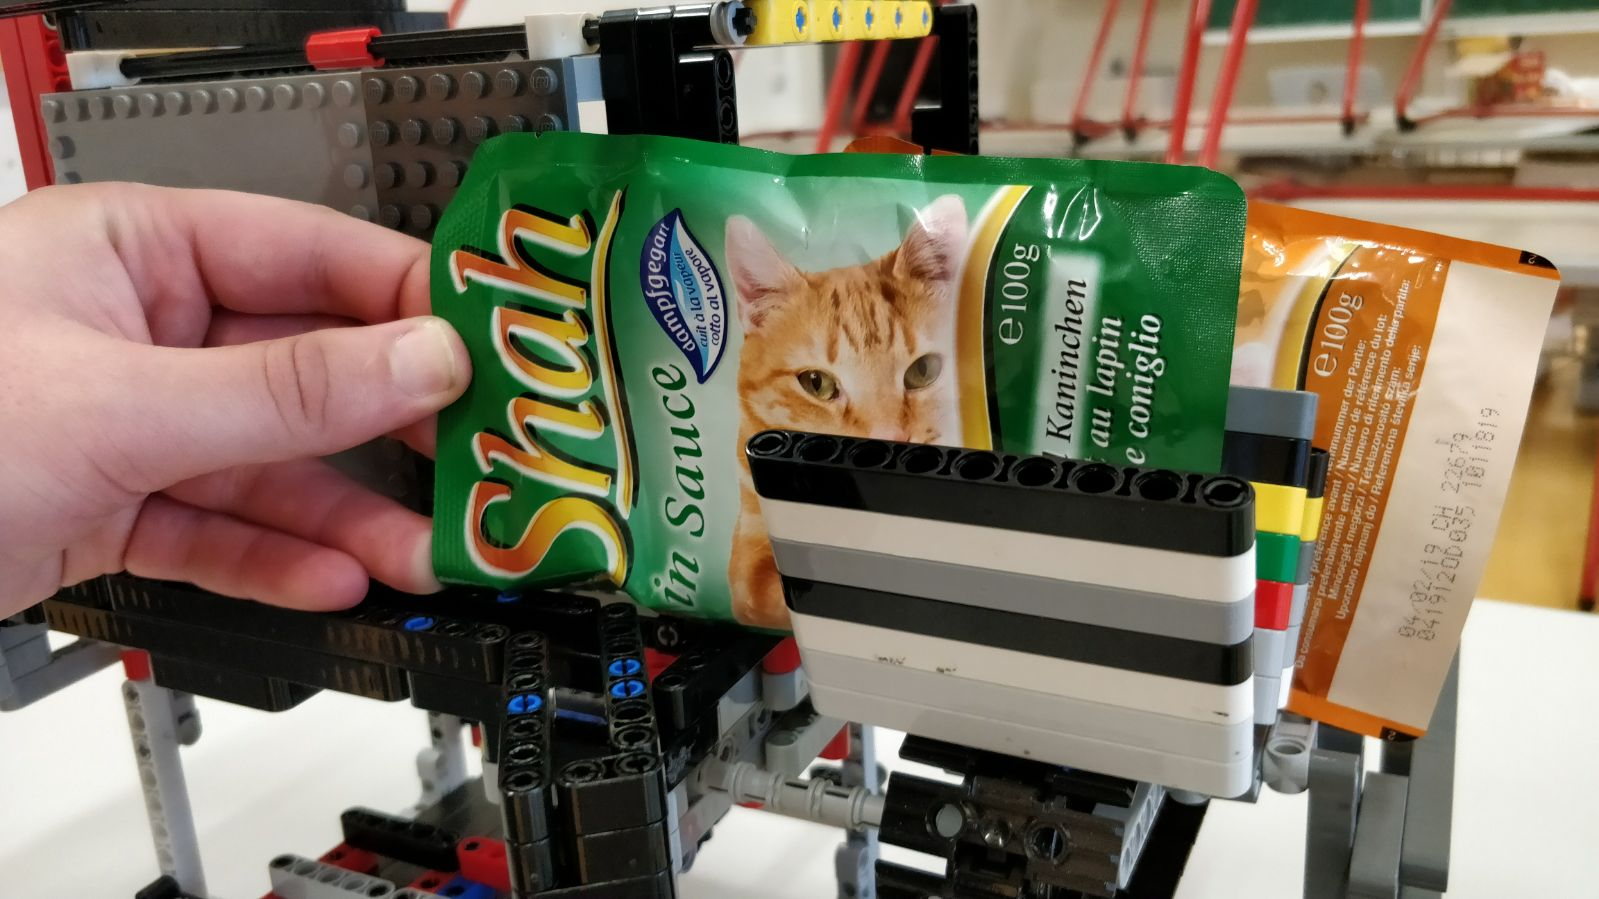
\includegraphics[width=13cm]{Bilder/Ablauf_1_png/Magazin_Auszug.jpeg}
\caption{Magazin Auszug}
\end{center}
\end{figure}

\begin{figure}[H]
\begin{center}
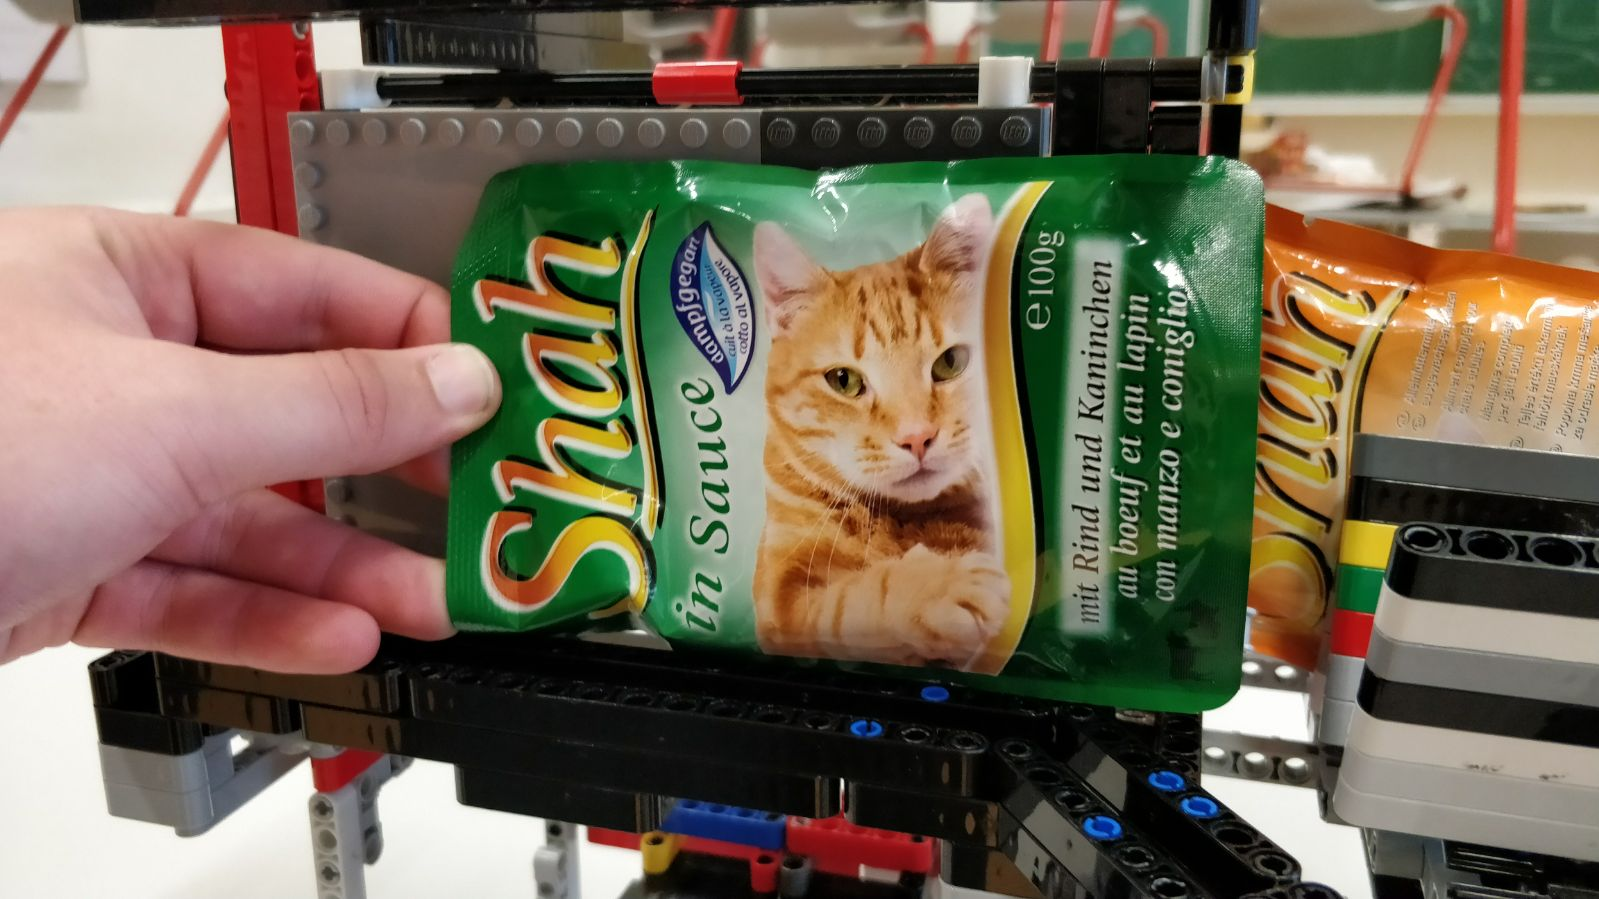
\includegraphics[width=13cm]{Bilder/Ablauf_1_png/Magazin_Auszug_2.jpeg}
\caption{Magazin Auszug 2}
\end{center}
\end{figure}

Wie im Bild gezeigt liegt das Katzenfutterpackerl in der richtigen Position und wird mit zwei Magnetzylindern an der Schneidefläche festgehalten.

\begin{figure}[H]
\begin{center}
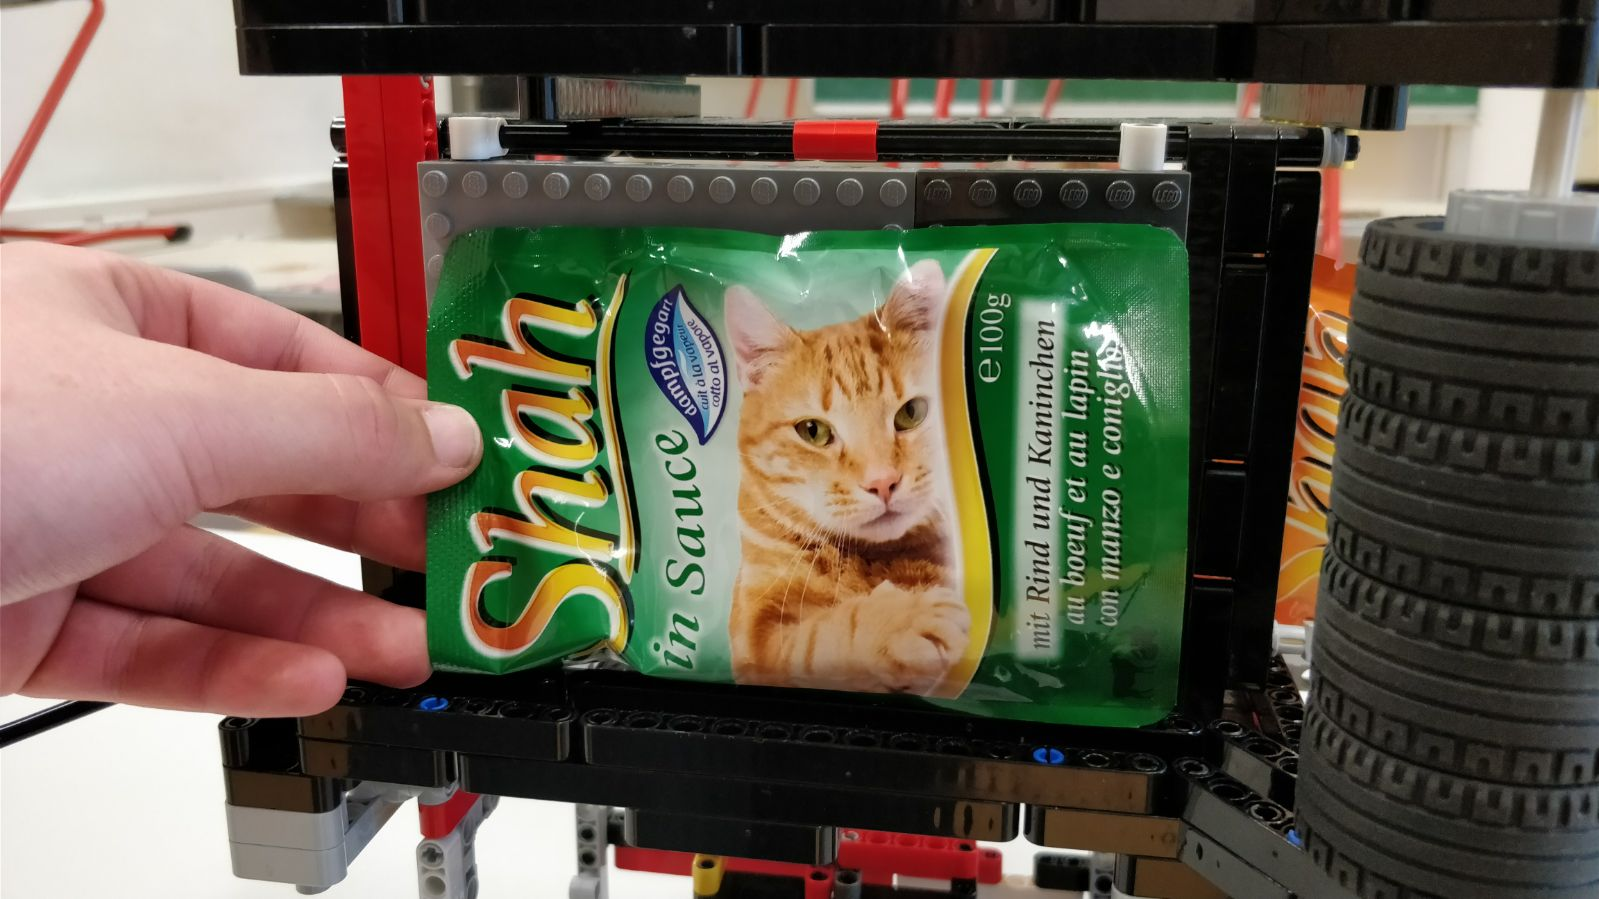
\includegraphics[width=13cm]{Bilder/Ablauf_1_png/Schneidebereit.jpeg}
\caption{Schneidebereit}
\end{center}
\end{figure}

Endposition des Greifers. Kerbe liegt genau an der richtigen Position. 4 Magnetzylinder halten den Futterbeutel and dieser Position, damit der Beutel während des Schneidens nicht verrutscht.

\begin{figure}[H]
\begin{center}
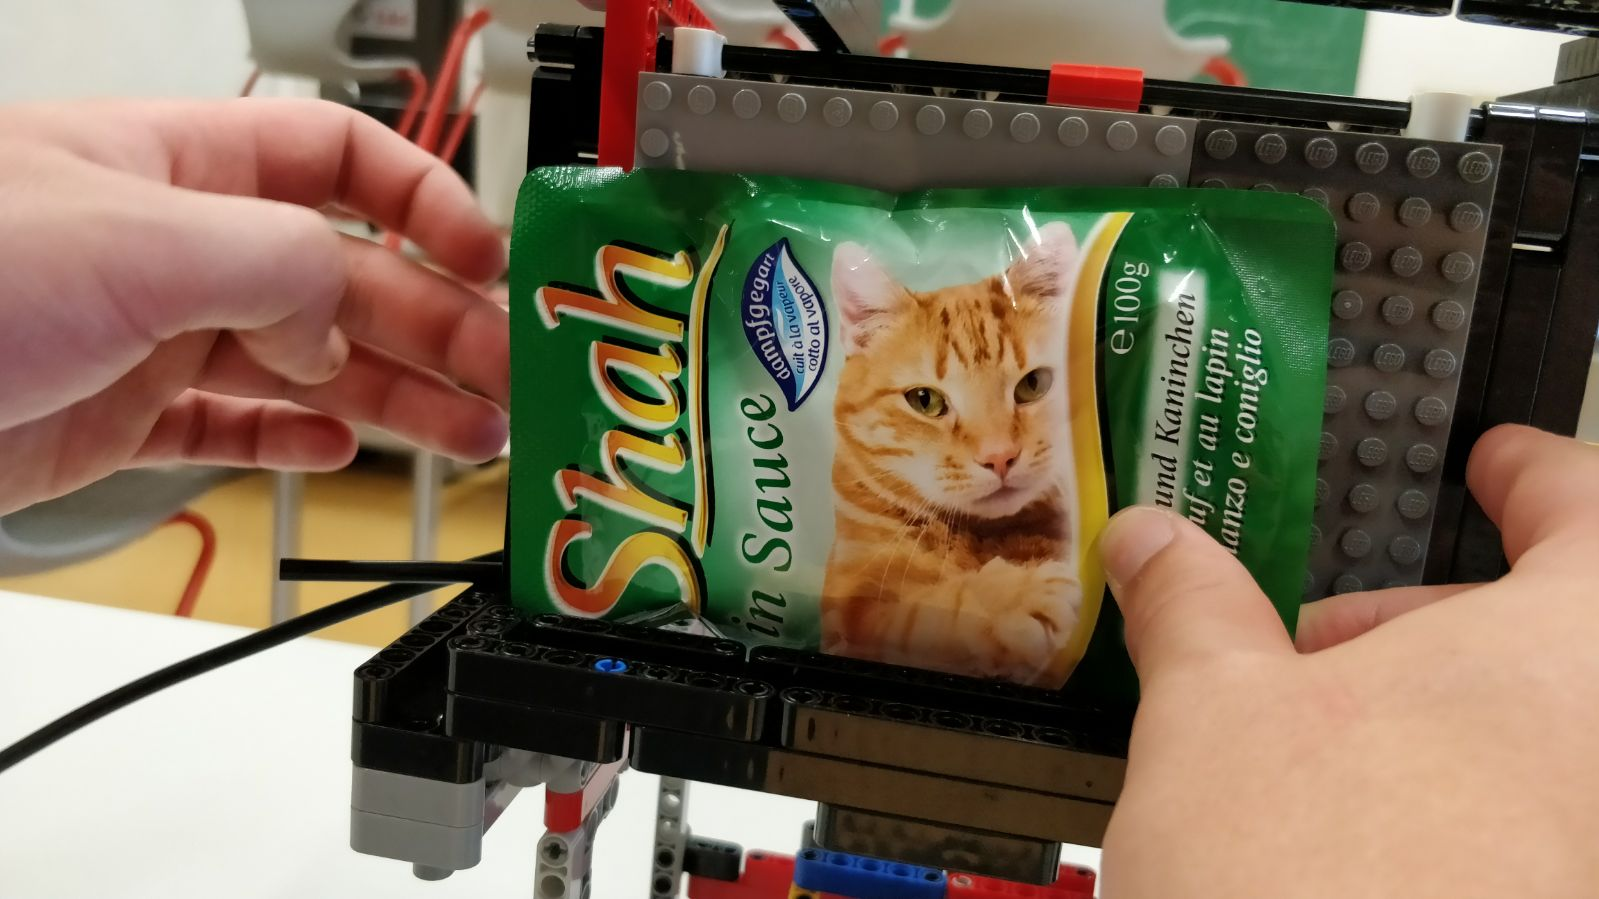
\includegraphics[width=13cm]{Bilder/Ablauf_1_png/Fertig_Geschnitten}
\caption{Fertig Geschnitten}
\end{center}
\end{figure}


\textbf{Schnitt:} \\

In der richtigen Position muss man mit 2 scharfen Klinge mit viel Druck die Packung aufschneiden. Eine davon wird and der Schnittfläche angebracht und die andere macht die Schneidbewegung, wobei die beiden aneinander reibenden Kanten in einem Schnitt resultieren. Die Packung kann mit einem Schnitt vollständig geöffnet werden.

Anhand dieses Bildes wird gezeigt wie der Schnitt funktionieren kann.

\begin{figure}[H]
\begin{center}
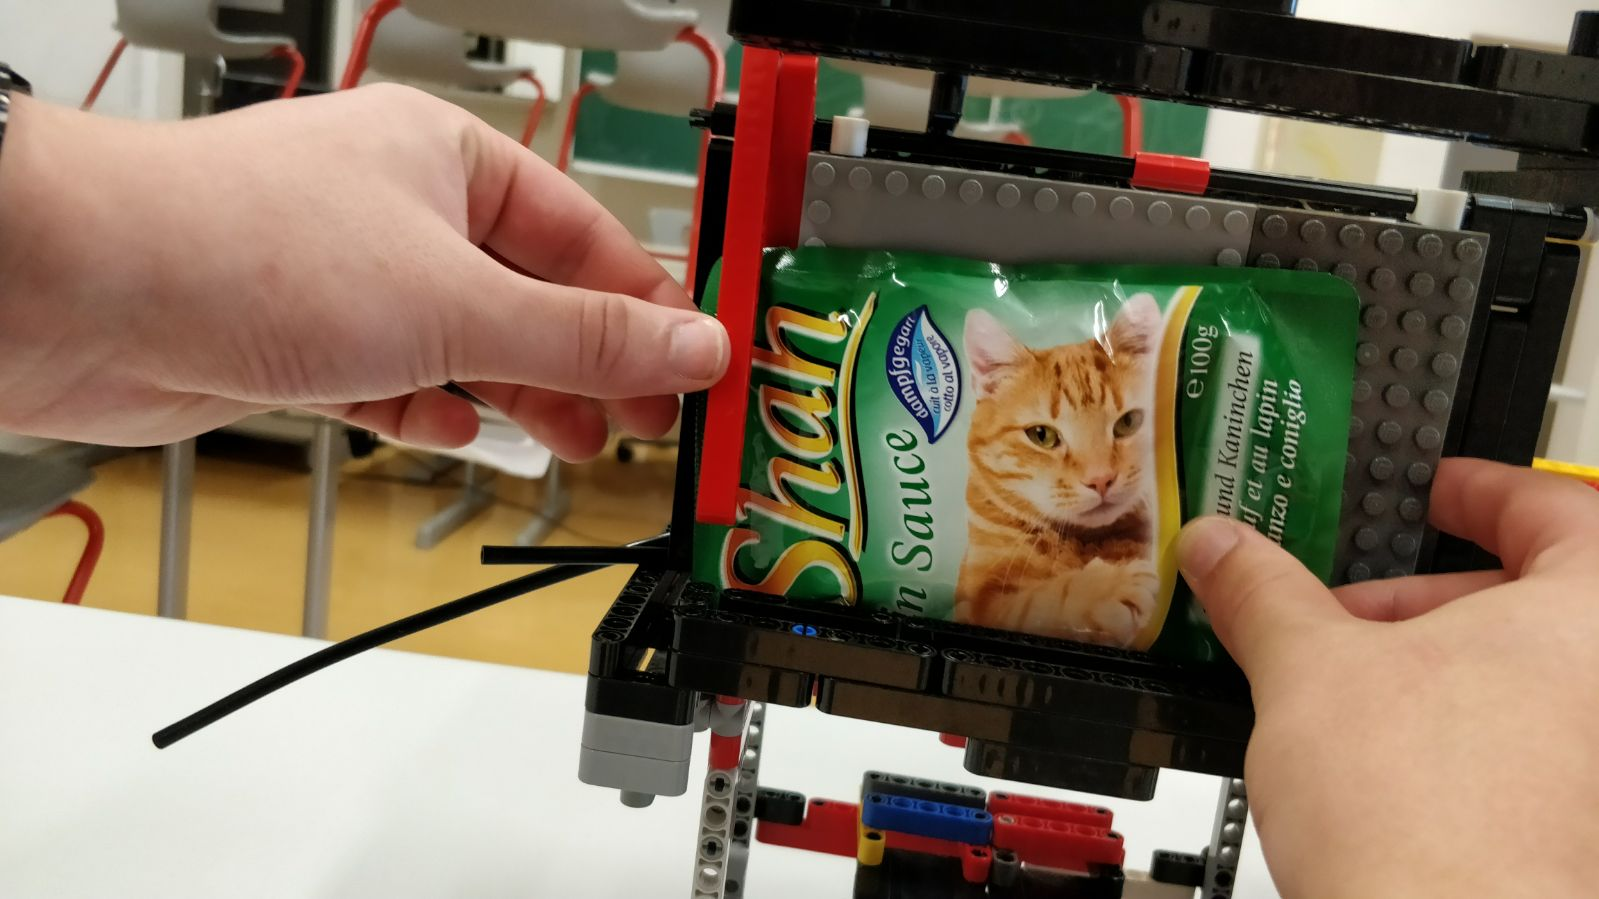
\includegraphics[width=13cm]{Bilder/Ablauf_1_png/Schnitt}
\caption{Fertig Geschnitten}
\end{center}
\end{figure}

Schnitt anhand einer praxischen Anwendung dargestellt. Der Beutel wird mithilfe einer Papierschneidemaschine geschnitten.

\begin{figure}[H]
\begin{center}
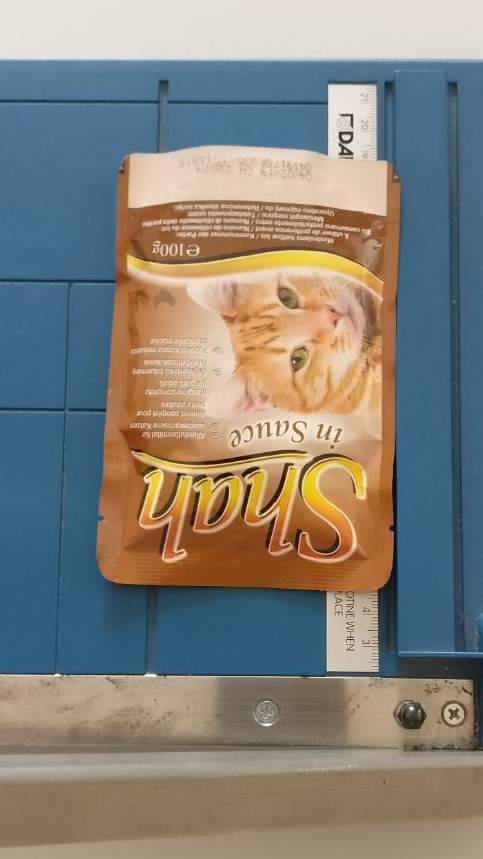
\includegraphics[width=5cm]{Bilder/Schneideversuch_1.Art/Einlegen}
\caption{Schnitt}
\end{center}
\end{figure}

\subsection{Aufbauten und Tests}
\subsection{Vergleich der Varianten}
\subsection{Konstruktion der Wahlvariante und Details}
\subsection{Berechnung und Dimensionierung}
\subsection{Simulation}
\subsection{Bedienung und Wartung}
\subsection{Selbstkritische Analyse und Ausblick}


\end{document}
